

\chapter{User-level Description}

\label{chap:userLevelDescription}
\section{Starting the Dash Line Plot Graphing Utility}


The application is distributed

\begin{itemize}
  \item either as a Python script, i.e. \texttt{dash-lineplot.py},
  \item or as an executable file, i.e. \texttt{dash-lineplot.exe}.
\end{itemize}

Double-clicking on any one of these files will start the application.
If the computer is not set up to associate \texttt{.py} files with the Python interpreter, open a windows command prompt window and type the following:

\footnotesize
\begin{lstlisting}
  python dash-lineplot.py
\end{lstlisting}
\normalsize

Working in a command prompt window is recommended. Warning and error messages output to the screen are published to the console. This can aid in tracing unexpected errors.

Working in an environment where the script was packaged to an executable, start the application from a console by typing

\footnotesize
\begin{lstlisting}
  dash-lineplot.exe
\end{lstlisting}
\normalsize

An easy, and recommended way of opening a command prompt at the correct folder location, is by following the steps:

\begin{itemize}
  \item Open the File Explorer.
  \item Navigate to the folder where the application Python script or executable is housed.
  \item Click in die File Explorer address bar.
  \item Type \texttt{cmd} into the address bar.
  \item Hit enter.
\end{itemize}

Hint: See 
\footnotesize
\url{https://www.howtogeek.com/235101/10-ways-to-open-the-command-prompt-in-windows-10/} \normalsize
for other ways to open a command prompt on Windows 10.

For ease of use a Windows batch script, \texttt{startPlotTool.bat}, is available in both environments. This script simply encapsulates the above commands:

\footnotesize
\begin{lstlisting}
    @echo off

    echo Starting the Dash Line Plot Graphing Tool ...
    echo.
    echo.

    if [%1]==[] python dash-lineplot.py
    if not [%1]==[] python dash-lineplot.py --configfile=%1

    set /p DUMMY=done, hit ENTER to exit
\end{lstlisting}
\normalsize

or

\footnotesize
\begin{lstlisting}
    @echo off

    echo Starting the Dash Line Plot Graphing Tool ....
    echo.
    echo.

    cd dash-lineplot

    if [%1]==[] dash-lineplot.exe
    if not [%1]==[] dash-lineplot.exe --configfile=%1

    set /p DUMMY=done, hit ENTER to exit
\end{lstlisting}
\normalsize


Starting the script with no commandline arguments results in loading the default \texttt{dash-config.xlsx} configuration file. A configuration file name can be specified on the commandline, using any of the following options:

\footnotesize
\begin{lstlisting}
  python dash-lineplot.py --configfile=anotherFileName.xlsx

  dash-lineplot.exe --configfile=anotherFileName.xlsx
  
  startPlotTool.bat anotherFileName.xlsx

\end{lstlisting}
\normalsize

Note that using the packaged version, the batch file starting the application is distributed at one folder level up from the actual distribution. This is done to give easy access to the script. The configuration file must be specified relative to the actual distribution folder. Figure~\ref{fig:folderdistEx} shows the position of the startup script relative to the distribution folder. In the script the directory is changed to the \texttt{dash-lineplot} folder and only then is the executable started. The configuration file is therefore always found on the path relative to folder \texttt{dash-lineplot}.

\begin{figure}[h]
\centering
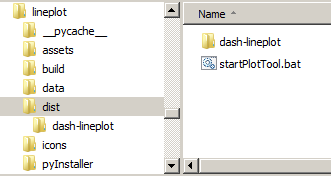
\includegraphics[width=0.5\textwidth]{pic/folderDistEx}
\caption{Distribution folder structure showing the location of the startup batch script.
\label{fig:folderdistEx}}
\end{figure}


\section{Setup and Usage}


\subsection{Configuration File and Page Layout}

Figures~\ref{fig:dashviewConfig1} and \ref{fig:dashviewConfig2} show the documentation sheet of the Excel plotting configuration file. A short description of variables are provided on this sheet. Refer to the information presented in these figures, no further details are provided in this document.

\begin{figure}[h]
\centering
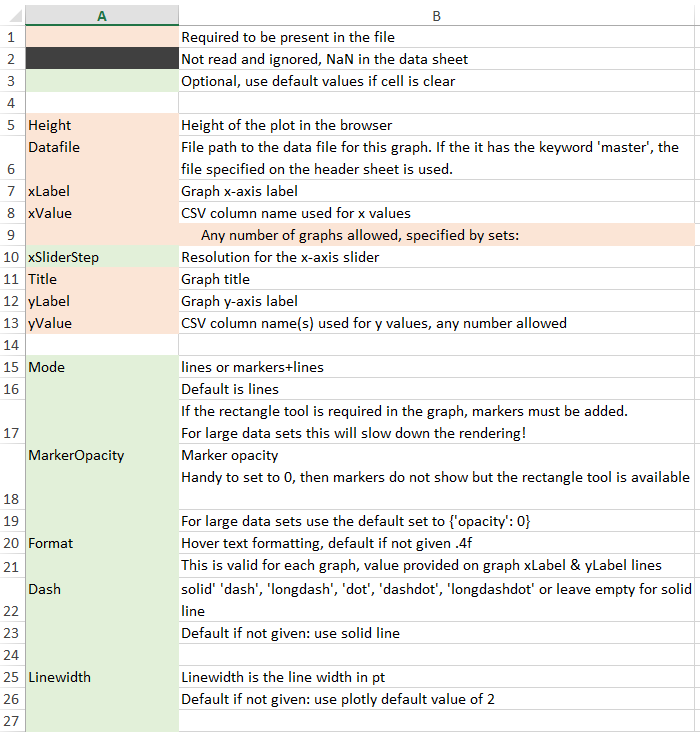
\includegraphics[width=0.90\textwidth]{pic/dashview-config1}
\caption{Documentation sheet of the Excel plotting configuration file.
\label{fig:dashviewConfig1}}
\end{figure}

\begin{figure}[h]
\centering
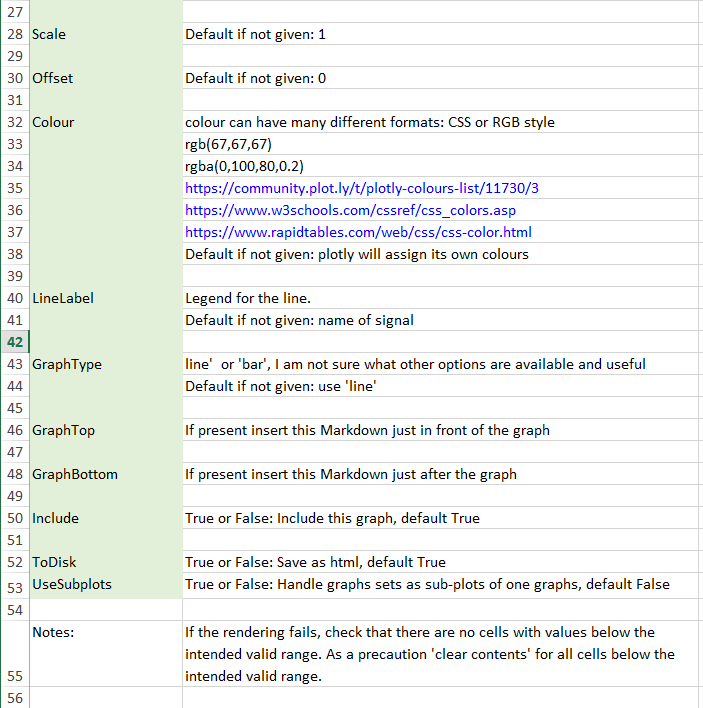
\includegraphics[width=0.90\textwidth]{pic/dashview-config2}
\caption{Documentation sheet of the Excel plotting configuration file (continued).
\label{fig:dashviewConfig2}}
\end{figure}

The header sheet in the configuration file, see annotated Figure~\ref{fig:dashview-config-header}, provides general information published on each page of the display. The user can provide a data file name on this sheet for general use. Sheets can refer to this file with the keyword \texttt{master} in the \texttt{Datafile} \texttt{Value} entry.

\begin{figure}[h]
\centering
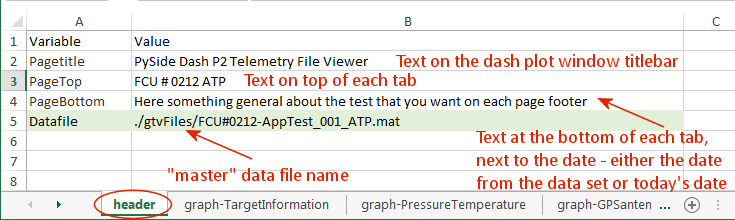
\includegraphics[width=0.90\textwidth]{pic/dashview-config-header}
\caption{Header sheet in the configuration file.
\label{fig:dashview-config-header}}
\end{figure}

Figures~\ref{fig:dashview-config-oscPL45} and \ref{fig:dashview-config-imuRates} are two example setup sheets specifying data configuration for plotting. The setup shown in Figure~\ref{fig:dashview-config-oscPL45} results in each set of traces to be plotted on a separate Plotly figure. The setup in Figure~\ref{fig:dashview-config-imuRates} makes use of Plotly subplots. Using subplots enables hover data on traces to be displayed simultaneously for all traces defined on the sheet, see example in Figure~\ref{fig:dashview-imuRates}. Exactly the same graph set plotted without the use of subplot is shown in Figure~\ref{fig:dashview-config-imuRates-noSubplots}.

\begin{figure}[h]
\centering
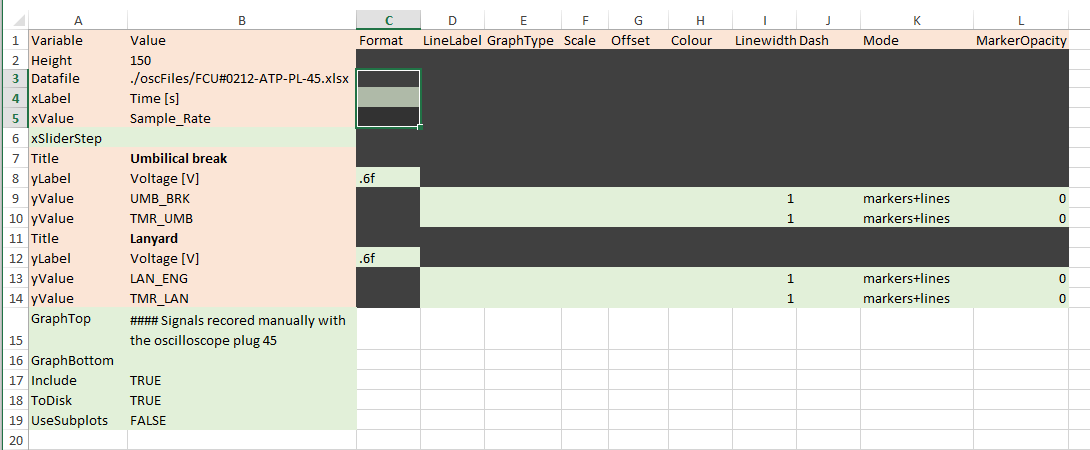
\includegraphics[width=\textwidth]{pic/dashview-config-oscPL45}
\caption{Example graph setup where subplots are not used, transparent markers are used and hover data format is specified.
\label{fig:dashview-config-oscPL45}}
\end{figure}
\begin{figure}[h]
\centering
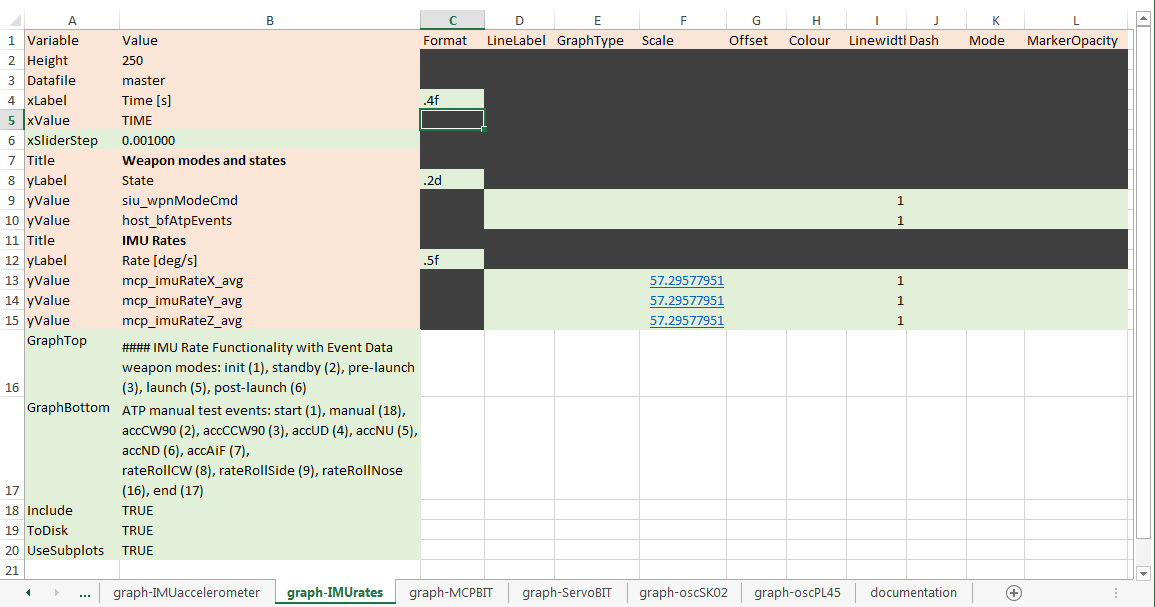
\includegraphics[width=\textwidth]{pic/dashview-config-imuRates}
\caption{Example setup where subplots are used, the IMU rates are scaled, no markers are used and hover data format is specified.
\label{fig:dashview-config-imuRates}}
\end{figure}

Figure~\ref{fig:dashview-imuRates} links the entries in the configuration file (refer to Figure~\ref{fig:dashview-config-imuRates}) to the format of the graph page. Note the following:

\begin{itemize}
  \item The tab name corresponds to the sheet name in the configuration file, omitting the leading \texttt{graph-} phrase.
  \item The header and footer at the top and bottom of the page are from the \texttt{header} sheet.
  \item The text entries just below and above these are the \texttt{GraphTop} and \texttt{GraphBottom} \texttt{Value} entries on the sheet.
  \item Two sets of traces are defined on the sheet, using subplots. Usage of the subplot option enables hover data to be displayed on all traces simultaneously.
  \item The hover data format is specified for the x-axis and two y-axis separately.
  \item The subplot titles, y-axis and x-axis labels are as provided in the \texttt{graph-IMUrates} sheet of the configuration file.
\end{itemize}

The same data is displayed in Figure~\ref{fig:dashview-config-imuRates-noSubplots}, not using the subplot functionality.

\begin{figure}[h]
\centering
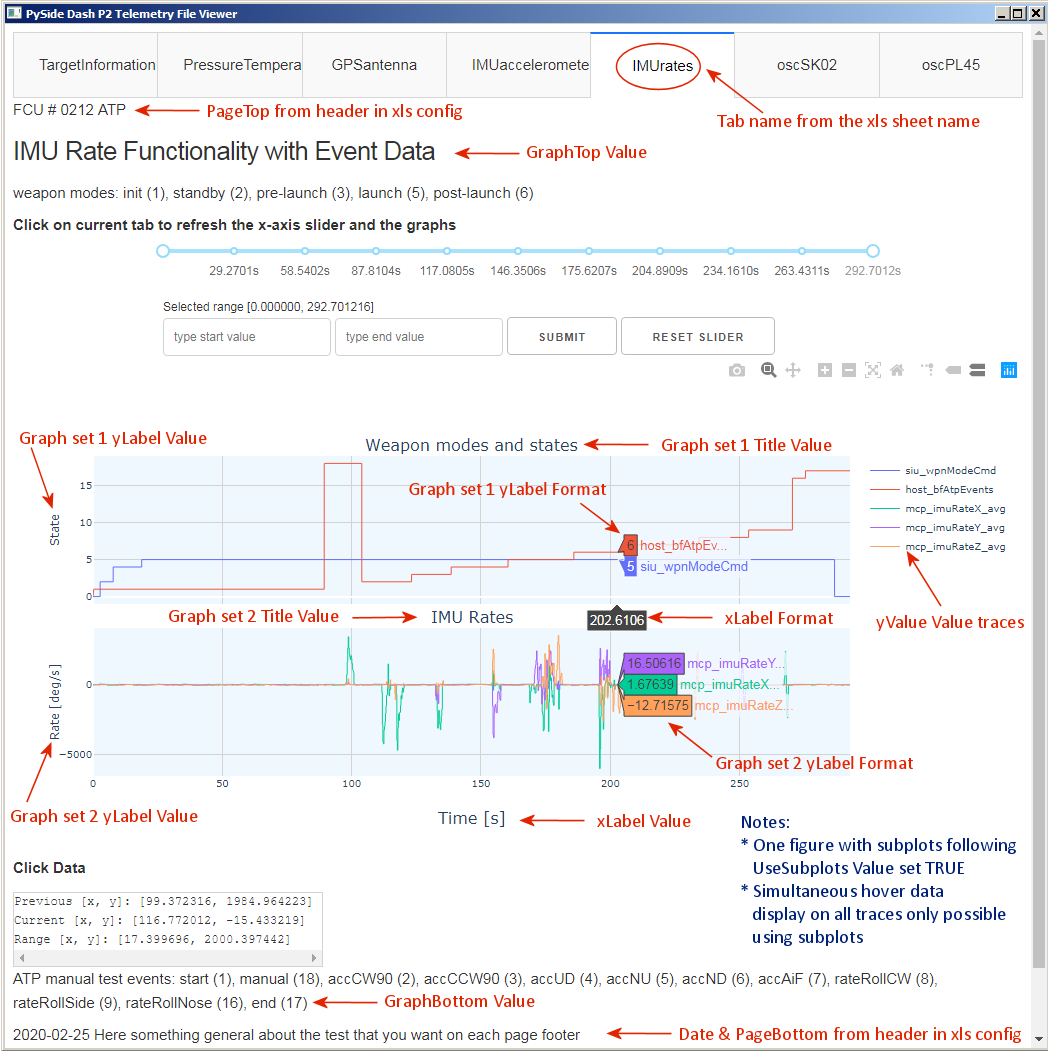
\includegraphics[width=\textwidth]{pic/dashview-imuRates}
\caption{Plot tab the IMU rates graph setup example, using subplots.
\label{fig:dashview-imuRates}}
\end{figure}


\begin{figure}[h]
\centering
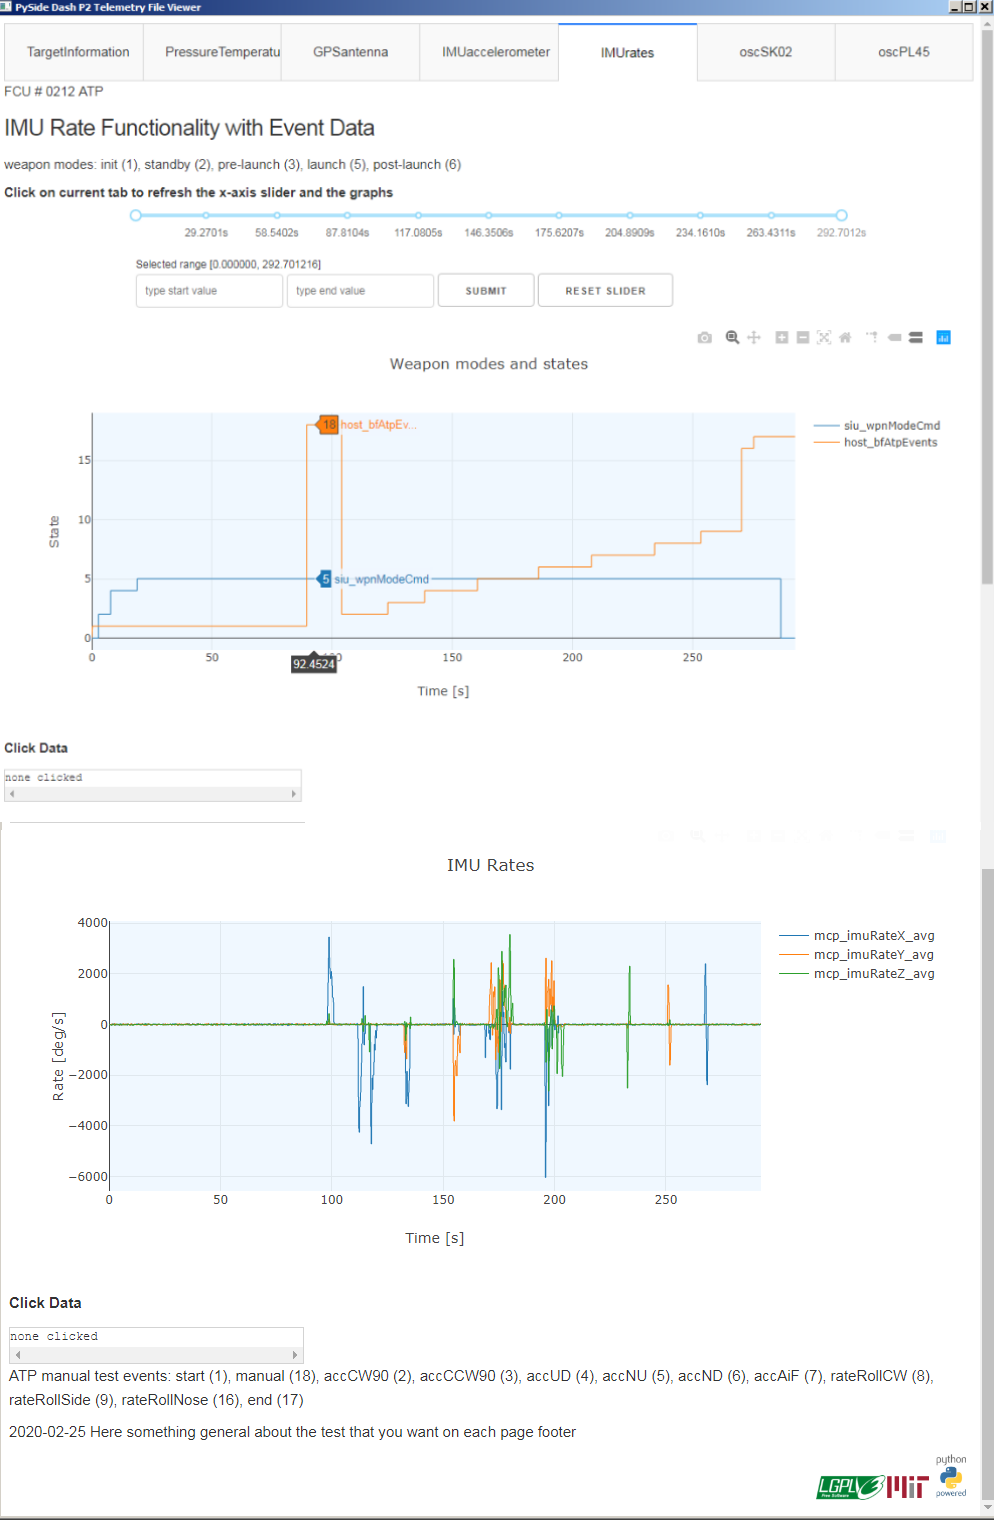
\includegraphics[height=0.95\textheight]{pic/dashview-config-imuRates-noSubplots}
\caption{Plot tab the IMU rates graph setup example, not using subplots.
\label{fig:dashview-config-imuRates-noSubplots}}
\end{figure}

\clearpage
\subsection{Slider Usage}

An x-axis slider is available at the top of each page, covering the data set x-axis data range. Refer to Figure~\ref{fig:dashview-subPlot2Slider1}. The user sets the minimum and maximum value of the x-axis with the slider handles. The text box immediately displays the selected range. The increments at which the slider values change are controlled by the specification from the configuration file. The user however has to click on the current page tab before the graphs are redrawn to display only data in the selected x-axis range, see Figure~\ref{fig:dashview-subPlot2Slider2}. The reset button will reset the x-axis limits to that of the data set.

\begin{figure}[h]
\centering
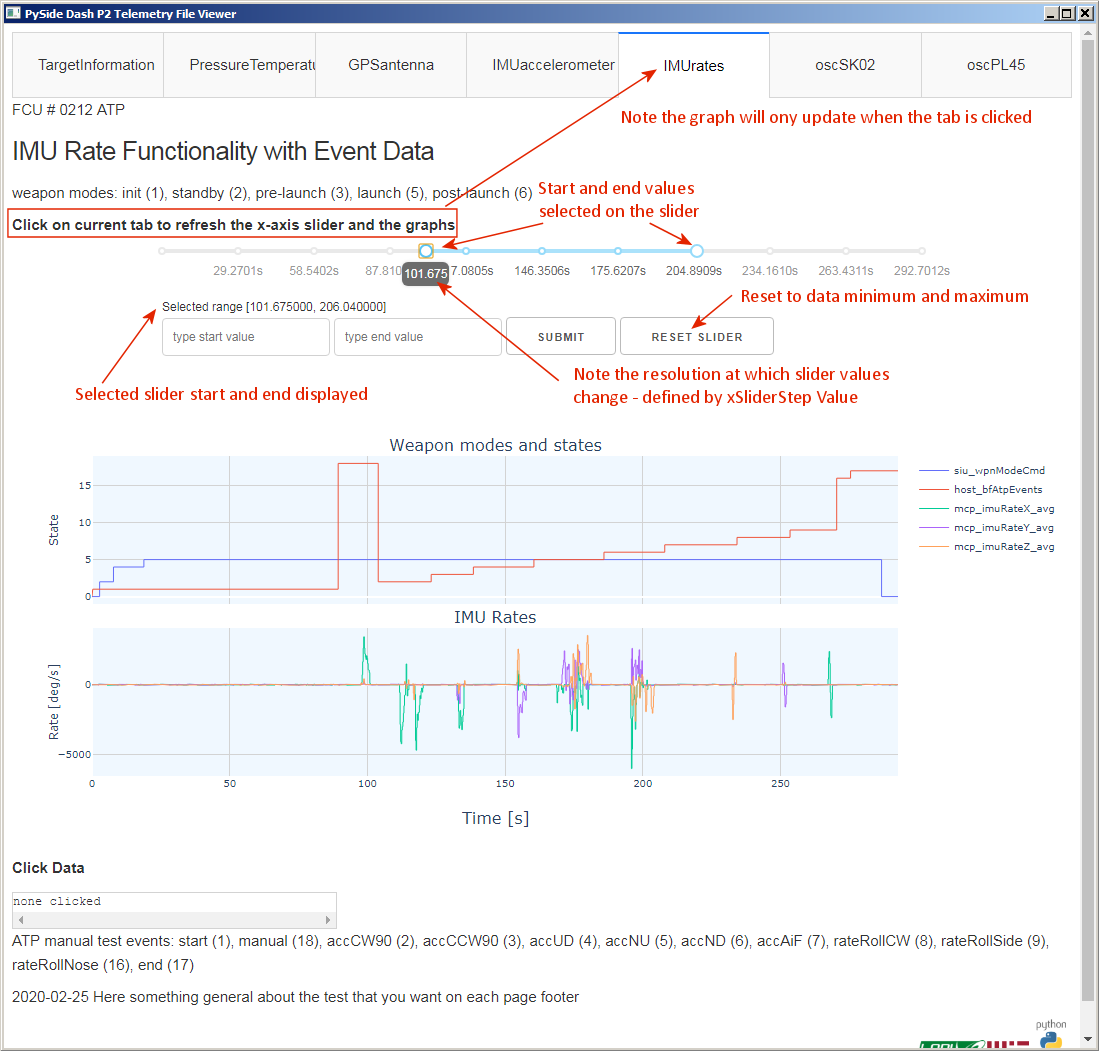
\includegraphics[width=\textwidth]{pic/dashview-subPlot2Slider1}
\caption{The x-axis slider at the top of the page provides the capability to zoom the complete data set to a user selected x-range.
\label{fig:dashview-subPlot2Slider1}}
\end{figure}

\begin{figure}[h]
\centering
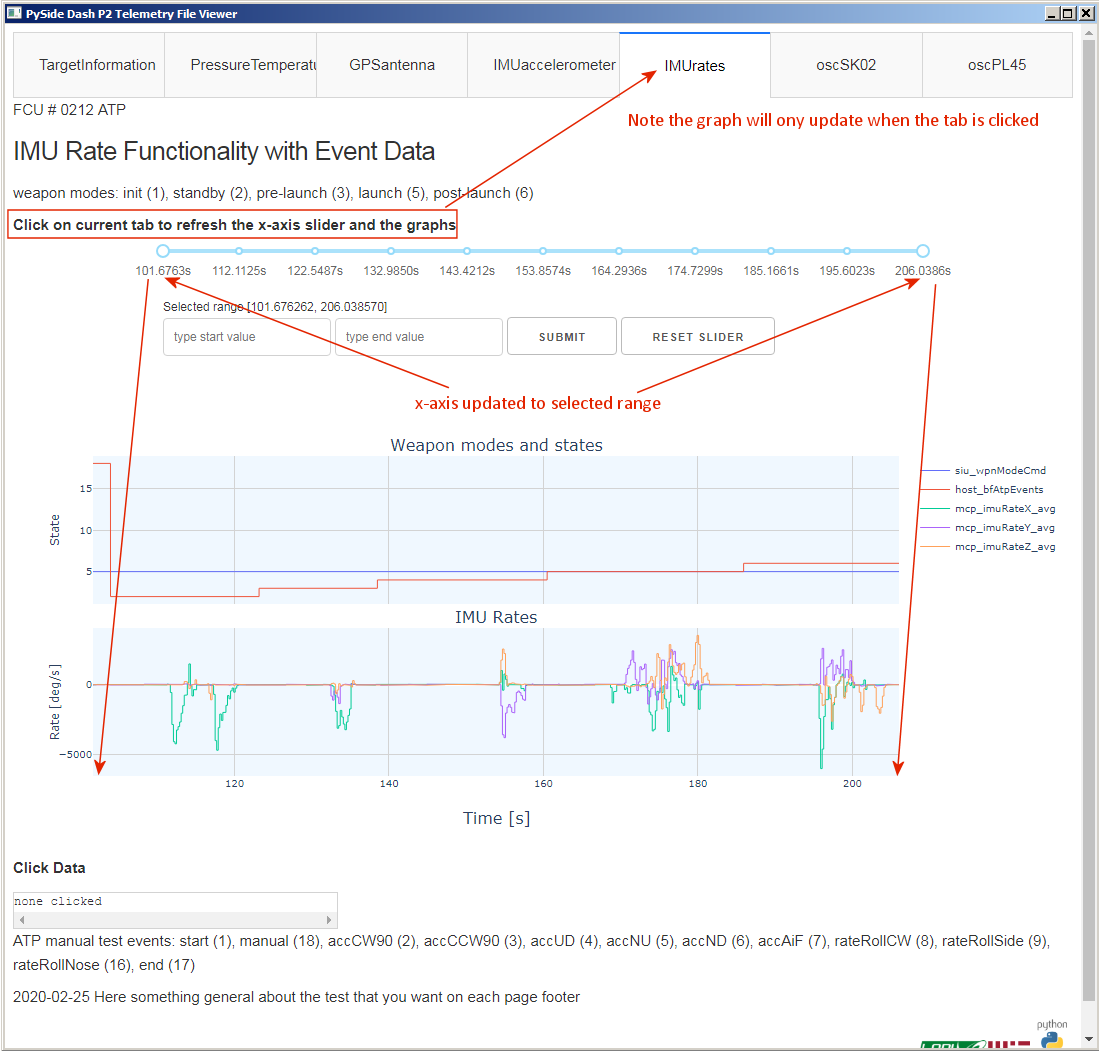
\includegraphics[width=\textwidth]{pic/dashview-subPlot2Slider2}
\caption{A click on the current page tab triggers the redraw of the page, using only data in the x-axis range selected by the user.
\label{fig:dashview-subPlot2Slider2}}
\end{figure}

\clearpage

The x-axis range can also be set by typing values in the text boxes just below the slider. Refer to Figure~\ref{fig:dashview-subPlot2Slider3}. The submit button records these selected values and activates the display of the selected range in the dedicated text box. A click on the tab will trigger an update to the graph data displayed.

\begin{figure}[h]
\centering
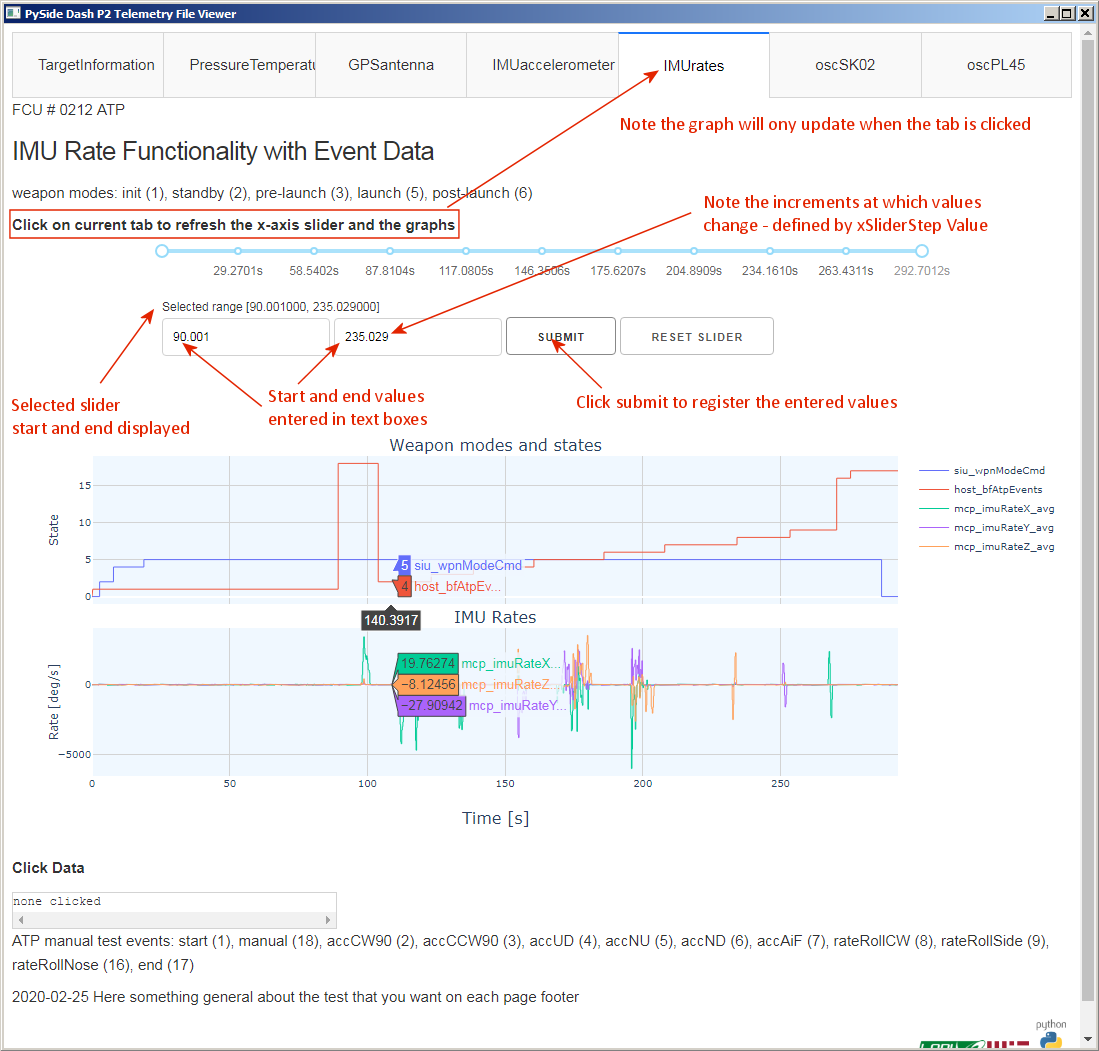
\includegraphics[width=\textwidth]{pic/dashview-subPlot2Slider3}
\caption{The user can specify the start and end values of the x-axis using the text boxes provided. The submit button will register the values for use when redrawing the graphs.
\label{fig:dashview-subPlot2Slider3}}
\end{figure}

\clearpage
\subsection{Range Measurements on Graphs}

Two methods are available to do a measurement on the graphs (see Figure~\ref{fig:dashview-rectangleDataSelect}):
\begin{description}
  \item [Click Data:] The user can click on any trace to record the clicked point in the \texttt{Click Data} box below the relevant graph. When a second data point is clicked, the range in x and y are reflected in the display text box. This functionality is available for individual Plotly figures, as well as subplot figures. The click functionality can be used in conjunction with the standard Plotly zoom functionality.
  \item [Rectangle Tool Selection Data:] The Plotly rectangle tool will only appear in the toolbar of the figure if markers are used for one or more traces in the figure. For large data sets, usage of this tool is not recommended since it slows down the drawing process. If the user prefers to use this tool, the opacity of the markers can be set to 0 in order to not clutter the graph. To measure using the rectangle tool, click on the tool in the toolbar, then draw the rectangle on the graph using the mouse. The top-left, bottom-right and range in x and y are displayed in the \texttt{Rectangle Tool Selection Data} text box to below the relevant graph. This functionality can also be used in conjunction with the Plotly zoom functionality.
\end{description}

\begin{figure}[h]
\centering
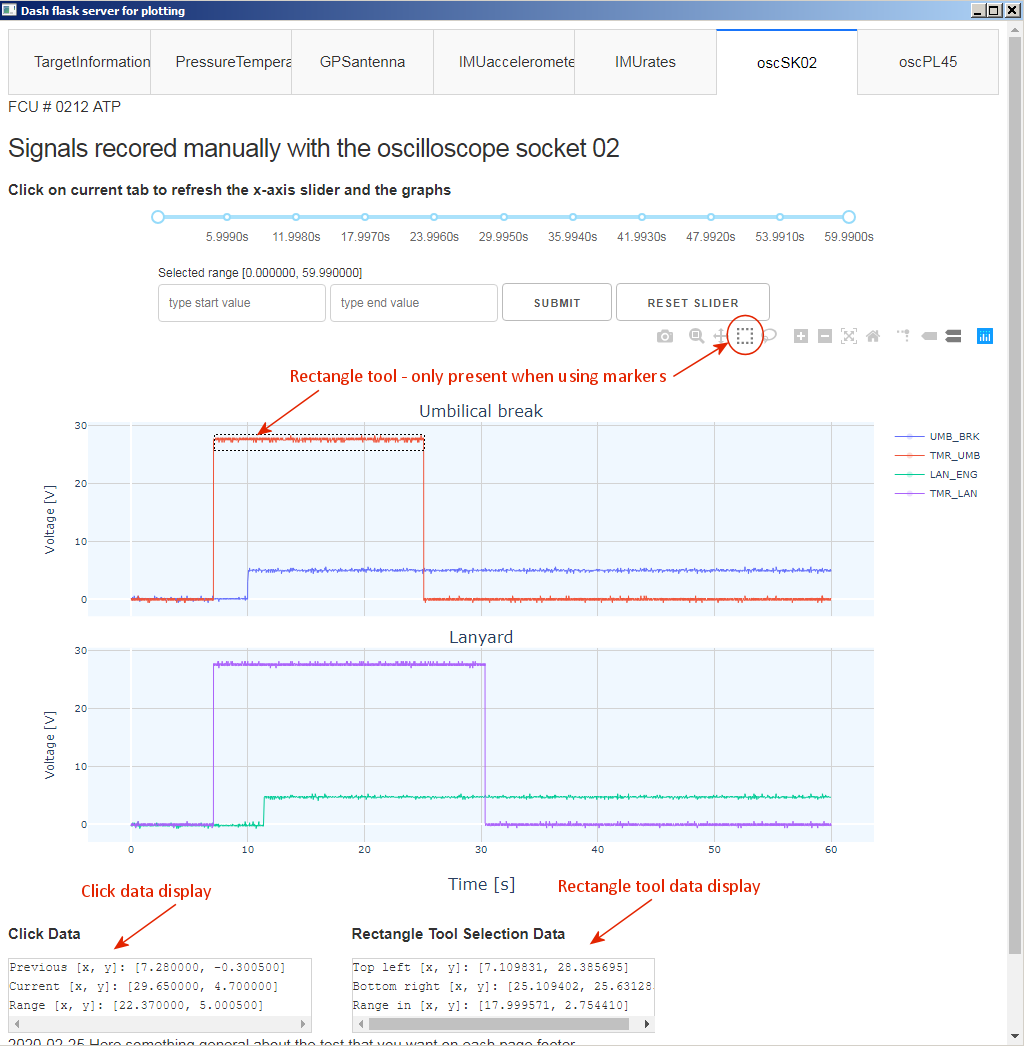
\includegraphics[width=\textwidth]{pic/dashview-rectangleDataSelect}
\caption{Using the Click and Rectangle tools to do measurements on the data set.
\label{fig:dashview-rectangleDataSelect}}
\end{figure}
